\documentclass[border=8pt]{standalone}
\usepackage[T1]{fontenc}\usepackage{helvet}\renewcommand{\familydefault}{\sfdefault}
\usepackage{tikz}\usetikzlibrary{arrows.meta, positioning, calc, backgrounds}
\definecolor{ink}{HTML}{1a1916}
\definecolor{inktwo}{HTML}{3a3a35}
\definecolor{inkthree}{HTML}{6a6862}
\definecolor{rule}{HTML}{b8b09a}
\definecolor{amber}{HTML}{a8730a}
\definecolor{red}{HTML}{c8261a}
\definecolor{paper}{HTML}{f0eee5}
\definecolor{slab}{HTML}{d8d4c6}
\tikzset{
  >={Stealth[length=2.2mm]},
  wire/.style={line width=0.8pt, ink},
  modwire/.style={line width=0.6pt, dashed, ink},
  tastewire/.style={line width=0.6pt, dashed, amber},
  gatewire/.style={line width=0.6pt, dotted, ink},
  block/.style={rectangle, draw=ink, line width=0.9pt, fill=slab, minimum width=3.0cm, minimum height=1.9cm, inner sep=0pt},
  perf/.style={rectangle, draw=ink, line width=0.7pt, minimum width=3.0cm, minimum height=0.7cm, inner sep=2pt, font=\footnotesize, text=ink},
  title/.style={font=\scriptsize\bfseries, text=ink, anchor=north, inner sep=2pt},
  jack/.style={circle, draw=ink, fill=paper, line width=0.5pt, minimum size=3.2pt, inner sep=0pt},
  plabel/.style={font=\tiny, text=inktwo, anchor=west, inner sep=1pt},
  olabel/.style={font=\tiny, text=inktwo, anchor=east, inner sep=1pt},
  settings/.style={font=\scriptsize, text=ink, align=left, anchor=north west, inner sep=1pt, text width=2.9cm},
}
\begin{document}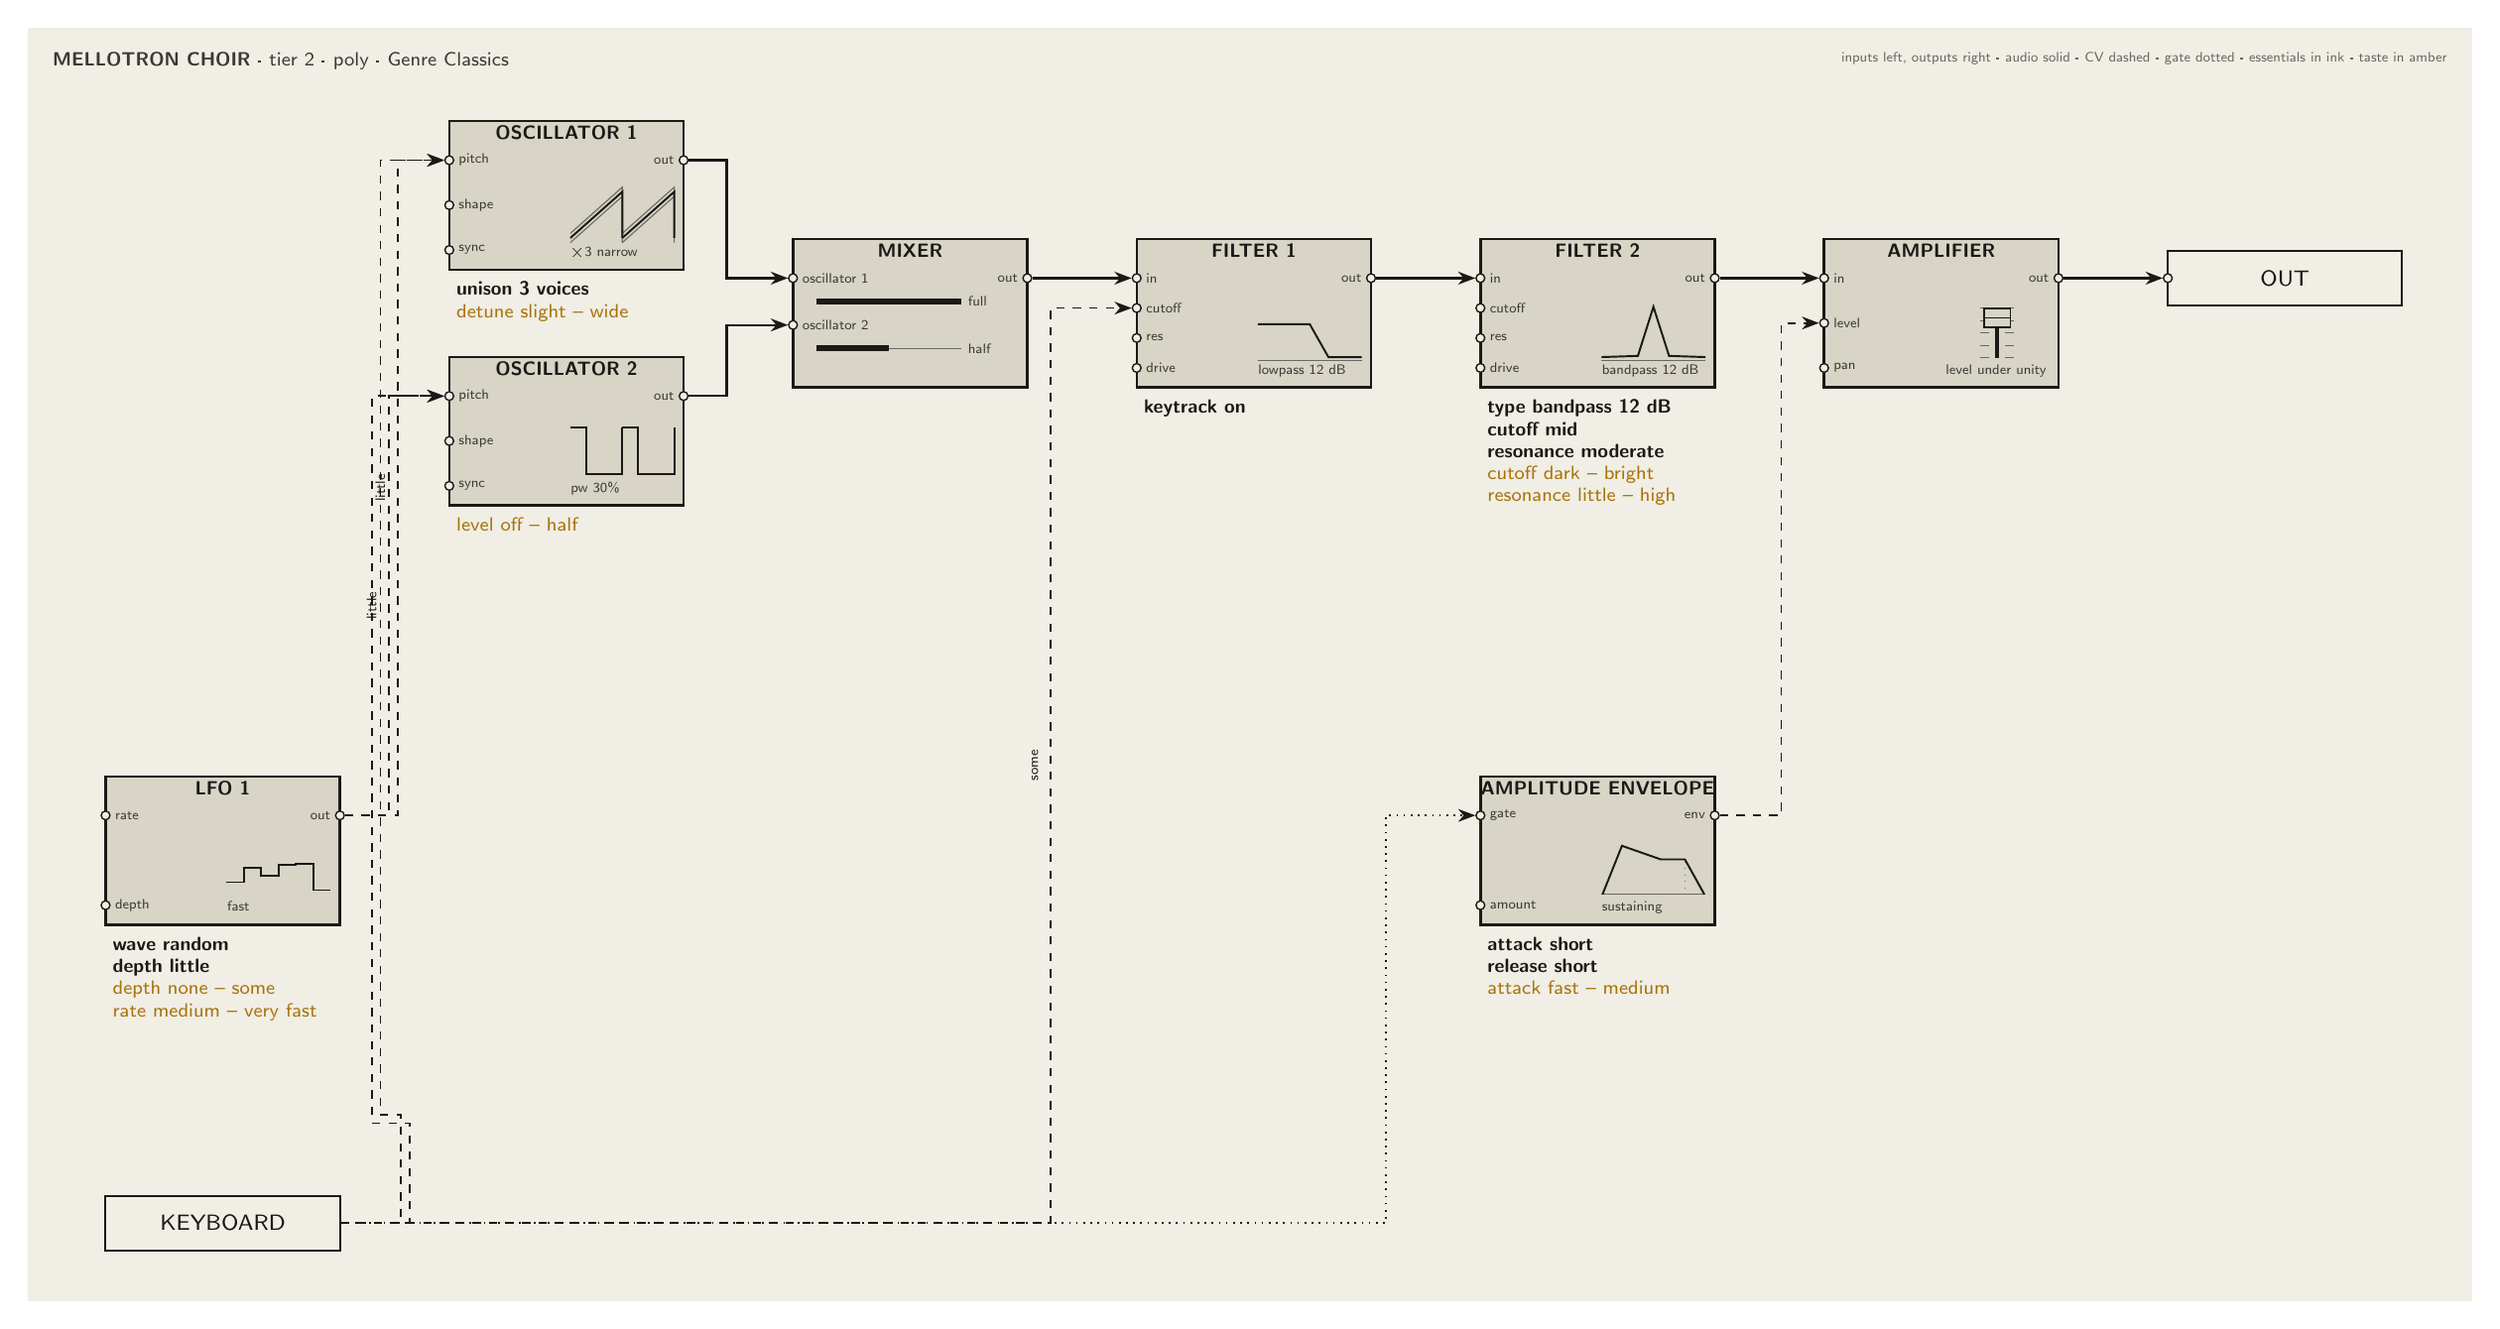
\begin{tikzpicture}
\begin{scope}[on background layer]\fill[paper] (-2.5,-12.649999999999999) rectangle (28.8,3.66);\end{scope}
\node[block, minimum height=1.9cm] (osc1) at (4.4,1.51) {};
\node[title] at (osc1.north) {OSCILLATOR 1};
\node[jack] (osc1-pitch) at (2.9000000000000004,1.96) {};
\node[plabel] at (2.9800000000000004,1.96) {pitch};
\node[jack] (osc1-shape) at (2.9000000000000004,1.385) {};
\node[plabel] at (2.9800000000000004,1.385) {shape};
\node[jack] (osc1-sync) at (2.9000000000000004,0.81) {};
\node[plabel] at (2.9800000000000004,0.81) {sync};
\node[jack] (osc1-out) at (5.9,1.96) {};
\node[olabel] at (5.82,1.96) {out};
\begin{scope}
\draw[inkthree, line width=0.4pt] (4.450,1.023) -- (5.115,1.615) -- (5.115,1.023);
\draw[inkthree, line width=0.4pt] (5.115,1.023) -- (5.780,1.615) -- (5.780,1.023);
\draw[inkthree, line width=0.4pt] (4.450,0.905) -- (5.115,1.497) -- (5.115,0.905);
\draw[inkthree, line width=0.4pt] (5.115,0.905) -- (5.780,1.497) -- (5.780,0.905);
\draw[ink, line width=0.7pt] (4.450,0.964) -- (5.115,1.556) -- (5.115,0.964);
\draw[ink, line width=0.7pt] (5.115,0.964) -- (5.780,1.556) -- (5.780,0.964);
\node[font=\tiny, text=inktwo, anchor=north west, inner sep=0pt] at (4.450,0.860) {×3 narrow};
\end{scope}
\node[settings] at (2.95,0.44000000000000006) {\textbf{unison 3 voices} \\ \textcolor{amber}{detune slight -- wide}};
\node[block, minimum height=1.9cm] (osc2) at (4.4,-1.51) {};
\node[title] at (osc2.north) {OSCILLATOR 2};
\node[jack] (osc2-pitch) at (2.9000000000000004,-1.06) {};
\node[plabel] at (2.9800000000000004,-1.06) {pitch};
\node[jack] (osc2-shape) at (2.9000000000000004,-1.635) {};
\node[plabel] at (2.9800000000000004,-1.635) {shape};
\node[jack] (osc2-sync) at (2.9000000000000004,-2.21) {};
\node[plabel] at (2.9800000000000004,-2.21) {sync};
\node[jack] (osc2-out) at (5.9,-1.06) {};
\node[olabel] at (5.82,-1.06) {out};
\begin{scope}
\draw[ink, line width=0.7pt] (4.450,-1.464) -- (4.649,-1.464) -- (4.649,-2.056) -- (5.115,-2.056) -- (5.115,-1.464);
\draw[ink, line width=0.7pt] (5.115,-1.464) -- (5.315,-1.464) -- (5.315,-2.056) -- (5.780,-2.056) -- (5.780,-1.464);
\node[font=\tiny, text=inktwo, anchor=north west, inner sep=0pt] at (4.450,-2.160) {pw 30\%};
\end{scope}
\node[settings] at (2.95,-2.58) {\textcolor{amber}{level off -- half}};
\node[block, minimum height=1.9cm] (mix) at (8.8,0.0) {};
\node[title] at (mix.north) {MIXER};
\node[jack] (mix-osc1) at (7.300000000000001,0.44999999999999996) {};
\node[plabel] at (7.380000000000001,0.44999999999999996) {oscillator 1};
\draw[inkthree, line width=0.3pt] (7.600,0.150) -- (9.450,0.150);
\draw[ink, line width=2.2pt] (7.600,0.150) -- (9.450,0.150);
\node[font=\tiny, text=inktwo, anchor=west, inner sep=1pt] at (9.500,0.150) {full};
\node[jack] (mix-osc2) at (7.300000000000001,-0.15000000000000002) {};
\node[plabel] at (7.380000000000001,-0.15000000000000002) {oscillator 2};
\draw[inkthree, line width=0.3pt] (7.600,-0.450) -- (9.450,-0.450);
\draw[ink, line width=2.2pt] (7.600,-0.450) -- (8.525,-0.450);
\node[font=\tiny, text=inktwo, anchor=west, inner sep=1pt] at (9.500,-0.450) {half};
\node[jack] (mix-out) at (10.3,0.44999999999999996) {};
\node[olabel] at (10.22,0.44999999999999996) {out};
\node[block, minimum height=1.9cm] (filter1) at (13.200000000000001,0.0) {};
\node[title] at (filter1.north) {FILTER 1};
\node[jack] (filter1-in) at (11.700000000000001,0.44999999999999996) {};
\node[plabel] at (11.780000000000001,0.44999999999999996) {in};
\node[jack] (filter1-cutoff) at (11.700000000000001,0.06666666666666665) {};
\node[plabel] at (11.780000000000001,0.06666666666666665) {cutoff};
\node[jack] (filter1-res) at (11.700000000000001,-0.31666666666666665) {};
\node[plabel] at (11.780000000000001,-0.31666666666666665) {res};
\node[jack] (filter1-drive) at (11.700000000000001,-0.7) {};
\node[plabel] at (11.780000000000001,-0.7) {drive};
\node[jack] (filter1-out) at (14.700000000000001,0.44999999999999996) {};
\node[olabel] at (14.620000000000001,0.44999999999999996) {out};
\begin{scope}
\draw[inkthree, line width=0.3pt] (13.250,-0.605) -- (14.580,-0.605);
\draw[ink, line width=0.7pt] (13.250,-0.139) -- (13.915,-0.139) -- (14.154,-0.561) -- (14.580,-0.561);
\node[font=\tiny, text=inktwo, anchor=north west, inner sep=0pt] at (13.250,-0.650) {lowpass 12 dB};
\end{scope}
\node[settings] at (11.750000000000002,-1.0699999999999998) {\textbf{keytrack on}};
\node[block, minimum height=1.9cm] (filter2) at (17.6,0.0) {};
\node[title] at (filter2.north) {FILTER 2};
\node[jack] (filter2-in) at (16.1,0.44999999999999996) {};
\node[plabel] at (16.18,0.44999999999999996) {in};
\node[jack] (filter2-cutoff) at (16.1,0.06666666666666665) {};
\node[plabel] at (16.18,0.06666666666666665) {cutoff};
\node[jack] (filter2-res) at (16.1,-0.31666666666666665) {};
\node[plabel] at (16.18,-0.31666666666666665) {res};
\node[jack] (filter2-drive) at (16.1,-0.7) {};
\node[plabel] at (16.18,-0.7) {drive};
\node[jack] (filter2-out) at (19.1,0.44999999999999996) {};
\node[olabel] at (19.020000000000003,0.44999999999999996) {out};
\begin{scope}
\draw[inkthree, line width=0.3pt] (17.650,-0.605) -- (18.980,-0.605);
\draw[ink, line width=0.7pt] (17.650,-0.561) -- (18.116,-0.546) -- (18.315,0.083) -- (18.515,-0.546) -- (18.980,-0.561);
\node[font=\tiny, text=inktwo, anchor=north west, inner sep=0pt] at (17.650,-0.650) {bandpass 12 dB};
\end{scope}
\node[settings] at (16.150000000000002,-1.0699999999999998) {\textbf{type bandpass 12 dB} \\ \textbf{cutoff mid} \\ \textbf{resonance moderate} \\ \textcolor{amber}{cutoff dark -- bright} \\ \textcolor{amber}{resonance little -- high}};
\node[block, minimum height=1.9cm] (amp) at (22.0,0.0) {};
\node[title] at (amp.north) {AMPLIFIER};
\node[jack] (amp-in) at (20.5,0.44999999999999996) {};
\node[plabel] at (20.58,0.44999999999999996) {in};
\node[jack] (amp-level) at (20.5,-0.125) {};
\node[plabel] at (20.58,-0.125) {level};
\node[jack] (amp-pan) at (20.5,-0.7) {};
\node[plabel] at (20.58,-0.7) {pan};
\node[jack] (amp-out) at (23.5,0.44999999999999996) {};
\node[olabel] at (23.42,0.44999999999999996) {out};
\begin{scope}
\draw[ink, line width=1.2pt] (22.715,-0.570) -- (22.715,0.070);
\draw[inkthree, line width=0.3pt] (22.495,-0.570) -- (22.615,-0.570) (22.815,-0.570) -- (22.935,-0.570);
\draw[inkthree, line width=0.3pt] (22.495,-0.410) -- (22.615,-0.410) (22.815,-0.410) -- (22.935,-0.410);
\draw[inkthree, line width=0.3pt] (22.495,-0.250) -- (22.615,-0.250) (22.815,-0.250) -- (22.935,-0.250);
\draw[inkthree, line width=0.3pt] (22.495,-0.090) -- (22.615,-0.090) (22.815,-0.090) -- (22.935,-0.090);
\draw[inkthree, line width=0.3pt] (22.495,0.070) -- (22.615,0.070) (22.815,0.070) -- (22.935,0.070);
\fill[slab, draw=ink, line width=0.6pt] (22.545,-0.178) rectangle (22.885,0.062);
\draw[ink, line width=0.5pt] (22.545,-0.058) -- (22.885,-0.058);
\node[font=\tiny, text=inktwo, anchor=north west, inner sep=0pt] at (22.050,-0.650) {level under unity};
\end{scope}
\node[block, minimum height=1.9cm] (lfo1) at (0.0,-6.88) {};
\node[title] at (lfo1.north) {LFO 1};
\node[jack] (lfo1-rate) at (-1.5,-6.43) {};
\node[plabel] at (-1.42,-6.43) {rate};
\node[jack] (lfo1-depth) at (-1.5,-7.58) {};
\node[plabel] at (-1.42,-7.58) {depth};
\node[jack] (lfo1-out) at (1.5,-6.43) {};
\node[olabel] at (1.42,-6.43) {out};
\begin{scope}
\draw[ink, line width=0.7pt] (0.050,-7.285) -- (0.272,-7.285) -- (0.272,-7.104) -- (0.493,-7.104) -- (0.493,-7.207) -- (0.715,-7.207) -- (0.715,-7.068) -- (0.937,-7.068) -- (0.937,-7.056) -- (1.158,-7.056) -- (1.158,-7.387) -- (1.380,-7.387);
\node[font=\tiny, text=inktwo, anchor=north west, inner sep=0pt] at (0.050,-7.530) {fast};
\end{scope}
\node[settings] at (-1.45,-7.95) {\textbf{wave random} \\ \textbf{depth little} \\ \textcolor{amber}{depth none -- some} \\ \textcolor{amber}{rate medium -- very fast}};
\node[block, minimum height=1.9cm] (aenv) at (17.6,-6.88) {};
\node[title] at (aenv.north) {AMPLITUDE ENVELOPE};
\node[jack] (aenv-gate) at (16.1,-6.43) {};
\node[plabel] at (16.18,-6.43) {gate};
\node[jack] (aenv-amount) at (16.1,-7.58) {};
\node[plabel] at (16.18,-7.58) {amount};
\node[jack] (aenv-out) at (19.1,-6.43) {};
\node[olabel] at (19.020000000000003,-6.43) {env};
\begin{scope}
\draw[inkthree, line width=0.3pt] (17.650,-7.441) -- (18.980,-7.441);
\draw[ink, line width=0.7pt] (17.663,-7.441) -- (17.912,-6.819) -- (18.408,-6.993) -- (18.718,-6.993) -- (18.967,-7.441);
\draw[inkthree, line width=0.3pt, dotted] (18.718,-7.441) -- (18.718,-6.993);
\node[font=\tiny, text=inktwo, anchor=north west, inner sep=0pt] at (17.650,-7.530) {sustaining};
\end{scope}
\node[settings] at (16.150000000000002,-7.95) {\textbf{attack short} \\ \textbf{release short} \\ \textcolor{amber}{attack fast -- medium}};
\node[perf] (key) at (0.0,-11.649999999999999) {KEYBOARD};
\node[perf, fill=paper] (out) at (26.400000000000002,0.44999999999999996) {OUT}; \node[jack] (out-in) at (24.900000000000002,0.44999999999999996) {};
\draw[wire,->] (osc1-out) -- (6.45,1.96) |- (mix-osc1);
\draw[wire,->] (osc2-out) -- (6.45,-1.06) |- (mix-osc2);
\draw[wire,->] (mix-out) -- (filter1-in);
\draw[wire,->] (filter1-out) -- (filter2-in);
\draw[wire,->] (filter2-out) -- (amp-in);
\draw[wire,->] (amp-out) -- (out-in);
\draw[modwire,->] (aenv-out) -- (19.95,-6.43) -- (19.95,-0.125) -- (amp-level);
\draw[modwire,->] (lfo1-out) -- (2.2400000000000007,-6.43) -- (2.2400000000000007,1.96) -- (osc1-pitch);
\node[font=\tiny, text=ink, anchor=south, inner sep=1pt, rotate=90] at (2.1200000000000006,-2.235) {little};
\draw[modwire,->] (lfo1-out) -- (2.1300000000000003,-6.43) -- (2.1300000000000003,-1.06) -- (osc2-pitch);
\node[font=\tiny, text=ink, anchor=south, inner sep=1pt, rotate=90] at (2.0100000000000002,-3.745) {little};
\draw[modwire,->] (key.east) -- (2.28,-11.649999999999999) -- (2.28,-10.26) -- (2.0200000000000005,-10.26) -- (2.0200000000000005,1.96) -- (osc1-pitch);
\draw[modwire,->] (key.east) -- (2.39,-11.649999999999999) -- (2.39,-10.37) -- (1.9100000000000006,-10.37) -- (1.9100000000000006,-1.06) -- (osc2-pitch);
\draw[modwire,->] (key.east) -- (10.6,-11.649999999999999) -- (10.6,0.06666666666666665) -- (filter1-cutoff);
\node[font=\tiny, text=ink, anchor=south, inner sep=1pt, rotate=90] at (10.48,-5.791666666666666) {some};
\draw[gatewire,->] (key.east) -- (14.89,-11.649999999999999) -- (14.89,-6.43) -- (aenv-gate);
\node[anchor=north west, font=\scriptsize, text=inktwo] at (-2.3,3.46) {\textbf{MELLOTRON CHOIR} · tier 2 · poly · Genre Classics};
\node[anchor=north east, font=\tiny, text=inkthree] at (28.6,3.46) {inputs left, outputs right · audio solid · CV dashed · gate dotted · essentials in ink · taste in amber};
\end{tikzpicture}\end{document}
